\chapter{Introduction}
This course will provide an introduction to AI techniques and approach analyzed nowadays and to understand
the current state of art we have to provide an Timeline to see progress and discover done during the time,
so in figure \ref{img:timeline} we will see all important events related with AI.

\begin{figure}
    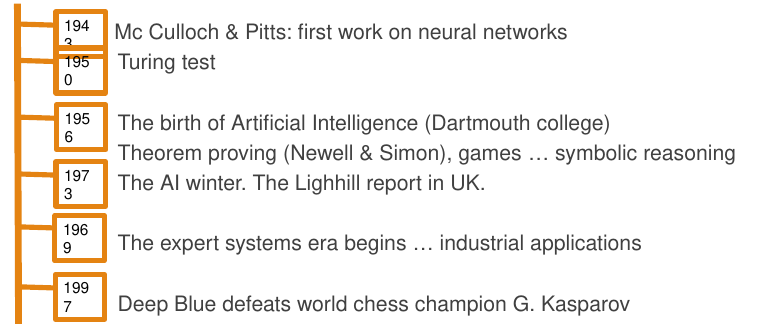
\includegraphics[width=0.45\textwidth]{Images/timeline}
    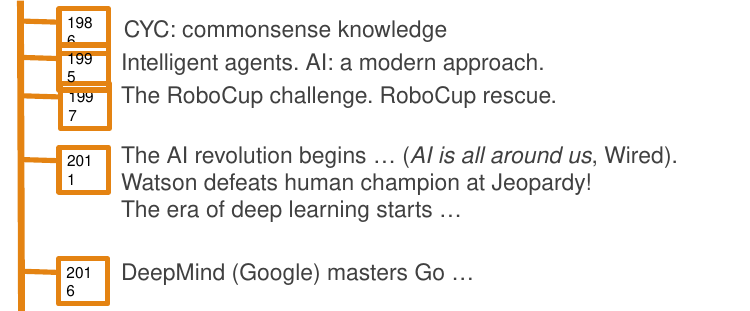
\includegraphics[width=0.45\textwidth]{Images/timeline2}
    \caption{AI Timeline evolution}
    \label{img:timeline}
\end{figure}
The major discover happened on $2020$ are the following:
\begin{description}
    \item [GPT3 (Generative Pre-trained Transformer): ] produced by OpenAI in May $2020$, is 
           a larger and richer language model consisting in $175$ billion machine learning parameters
           used for automatic text generation, translation, user interface synthesis
    \item [DARPA challenge (AlphaDogFights)] with simulated F-$16$ Air Fighters where on $18$-$20$ August $2020$
           there was the final Event, where AI system was against each other and the winner was a system by 
           Heron system, that was also able to defeated a human expert top gun fighter $5-0$.
\end{description}
Andrew NG says that AI will transform many industries, but it’s not magic and 
almost all of AI’s recent progress is based on one type of AI, in which some input data $(A)$ is used to
quickly generate some simple response $(B)$ [$A \to B$].\newline
Also Andrew Ng says that if a typical person can do a mental task with less than one second of thought,
we can probably automate it using AI either now or in the near future.\newline
Choosing A and B creatively has already revolutionized many industries, it is poised to
revolutionize many more.

ML systems are not (yet?) able to justify in human terms their results, so for some application it is essential
the human knowledge to be able to generate explanations, infact some regulations requires the right
to an explanation in decision-making, and seek to prevent discrimination based on race, opinions,
health, sex and so on, like GPDR.\newline
ML systems learn what’s in the data, without understanding what's true or false, real or imaginary, 
fair or unfair and so it is possible to develop bad/unfair models.

The goal of building AI systems is far from being solved and is still quite challenging in its own.
Building complex AI systems requires the combination of several techniques and approaches, not only ML.\newline
One of the most challenging tasks ahead of us is integration of
perception and reasoning in AI systems.

AI fundamentals is mostly about “Slow thinking” or “Reasoning” and AI fundamentals has the role,
within the AI curriculum, of teaching you about the foundations of a discipline which is now 60 year old.\newline
We will cover different approaches, also some coming of the “Good Old-
Fashioned Artificial Intelligence” (GOFAI) or symbolic AI.

\begin{defi}
Symbolic AI is an high-level "symbolic" (human-readable) representations of problems, the 
general paradigm of searching for a solution, knowledge representation and reasoning, planning.\newline
Symbolic AI was the dominant paradigm of AI research from the mid 1950s until the late 1980s and 
central to the building of AI systems is the \emph{Physical symbol systems hypothesis}, formulated by Newell and Simon.
\end{defi}

The approach is based on the assumption that many aspects of intelligence can be achieved by the 
manipulation of symbols (the physical symbol system hypothesis):
\begin{defi}
A physical symbol system has the necessary and sufficient means for general intelligent action
\end{defi}%CITE WHO SAYS THAT
Human thinking is a kind of symbol manipulation system (a symbol system is necessary for intelligence) and 
machines can be intelligent (a symbol system is sufficient for intelligence).\newline
The hypothesis cannot be proven, we can only collect empirical evidence and observations and experiments
on human behavior in tasks requiring intelligence.

We have two different typologies of AI, that was introduced and considered:
\begin{description}
    \item [Strong AI: ] relies on the strong assumption that human intelligence can be reproduced
                        in all its aspects (general A.I.).\newline
                        It includes adaptivity, learning, consciousness and not only pre-programmed behavior.
    \item [Weak AI: ]   simulation of human-like behavior, without effective thinking/understanding and 
                        no claim that it works like human mind; it is the dominant approach today.
\end{description}
A problem of AI is that computer can't have needs, cravings or desires and Abraham Maslow's define 
a hierarchy of human needs:
\begin{enumerate}
    \item Biological needs (food, sleep, sex, ...)
    \item Safety, protection from environment
    \item Love and belonging, friendship
    \item Self esteem and respect from others
    \item Self-actualization
\end{enumerate}
